\documentclass[11pt]{article}

% ====================================
% NEURIPS 2025 PROFESSIONAL TYPOGRAPHY
% ====================================

% Page geometry - NeurIPS standard
\usepackage[letterpaper, margin=1in]{geometry}

% Font packages - professional typography
\usepackage{times}                    % NeurIPS standard font
\usepackage[T1]{fontenc}             % Better font encoding
\usepackage{textcomp}                 % Additional text symbols
\usepackage{microtype}                % Microtypography for better text appearance

% Mathematics
\usepackage{amsmath,amssymb,amsfonts}
\usepackage{mathtools}                % Extended math functionality

% Tables and figures
\usepackage{graphicx}
\usepackage{booktabs}                 % Professional tables
\usepackage{array}                    % Better column specs

% Float control - Basic LaTeX has built-in controls

% Spacing and list control - available in BasicTeX

% Bibliography - NeurIPS-style citations
\usepackage[numbers,sort&compress]{natbib}
\bibliographystyle{plainnat}

% Hyperlinks - subtle formatting
\usepackage[colorlinks=true,
            linkcolor=darkblue,
            citecolor=darkblue,
            urlcolor=darkblue,
            bookmarks=true]{hyperref}
\usepackage{url}

% Colors
\usepackage{xcolor}
\definecolor{darkblue}{rgb}{0,0,0.5}

% ====================================
% TYPOGRAPHY SETTINGS
% ====================================

% Microtype settings for optimal typography
\microtypesetup{
    protrusion=true,
    expansion=true,
    final,
    tracking=false,
    kerning=true,
    spacing=true,
    factor=1100,
    stretch=10,
    shrink=10
}

% Float spacing - professional settings
\setlength{\floatsep}{12pt plus 2pt minus 2pt}
\setlength{\textfloatsep}{12pt plus 2pt minus 2pt}
\setlength{\intextsep}{12pt plus 2pt minus 2pt}
\setlength{\dblfloatsep}{12pt plus 2pt minus 2pt}
\setlength{\dbltextfloatsep}{12pt plus 2pt minus 2pt}

% Caption formatting - professional style
\usepackage[font=small,labelfont=bf,labelsep=period]{caption}
\captionsetup{
    format=plain,
    justification=justified,
    singlelinecheck=false,
    skip=6pt
}

% Section spacing - manual settings without titlesec
\makeatletter
\renewcommand\section{\@startsection{section}{1}{\z@}%
  {-18pt plus -4pt minus -2pt}%
  {10pt plus 2pt minus 1pt}%
  {\normalfont\Large\bfseries}}
\renewcommand\subsection{\@startsection{subsection}{2}{\z@}%
  {-12pt plus -3pt minus -1pt}%
  {6pt plus 1pt minus 0.5pt}%
  {\normalfont\large\bfseries}}
\makeatother

% Paragraph settings
\setlength{\parskip}{0pt}
\setlength{\parindent}{15pt}
\setlength{\parfillskip}{30pt plus 1fil}

% Prevent widows and orphans
\widowpenalty=10000
\clubpenalty=10000
\displaywidowpenalty=10000

% Better page breaks
\raggedbottom
\sloppy

% List formatting - manual without enumitem
\renewcommand{\@listI}{%
  \setlength{\topsep}{6pt}%
  \setlength{\itemsep}{3pt}%
  \setlength{\parsep}{0pt}%
  \setlength{\partopsep}{0pt}%
}

% ====================================
% CUSTOM COMMANDS
% ====================================

% For anonymous submission
\newcommand{\neuripsauthor}[1]{}
\newcommand{\neuripsaddress}[1]{}

% Mathematical notation
\newcommand{\R}{\mathbb{R}}
\newcommand{\E}{\mathbb{E}}
\newcommand{\Var}{\mathrm{Var}}
\DeclareMathOperator*{\argmin}{arg\,min}
\DeclareMathOperator*{\argmax}{arg\,max}

% ====================================
% DOCUMENT
% ====================================

\title{Proof-of-Training (PoT) Verifier: Cryptographically Pre-Committed,\\
Anytime Behavioral Model Identity Checks}

\date{}

\begin{document}

\maketitle

\begin{abstract}
We present a \textbf{post-training behavioral verifier} for model identity. 
Given two models (or a model and a reference), we decide 
\textbf{SAME/DIFFERENT/UNDECIDED} with \textbf{controlled error} using 
\textbf{dozens of queries} rather than thousands, with automatic 
\textbf{behavioral fingerprinting} for model variants. 
The verifier (i)~\textbf{pre-commits} to challenges via \textbf{HMAC-derived seeds}, 
(ii)~maintains \textbf{anytime confidence sequences} using 
\textbf{Empirical-Bernstein bounds}~\cite{maurer2009empiricalbernstein,howard2021timeuniform,howard2021confidenceSequences}, 
and (iii)~\textbf{stops early} when confidence intervals reach decision thresholds. 
Each run exports a \textbf{reproducible audit bundle} containing transcripts, 
seeds, commitments, configs, and environment data. 
On the systems side, we demonstrate \textbf{sharded verification} of 
\textbf{34B-class models} ($\approx$\textbf{206\,GB} weights) on \textbf{64\,GB} hosts 
with $\approx$\textbf{52\%} peak RAM usage through shard cycling. 
The repository includes \textbf{single-command runners} for both \textbf{local} 
and \textbf{API-based} verification. 
PoT fully verifies API-hosted models; \textbf{provider authentication} 
(proving server operator identity) requires separate infrastructure like 
\textbf{TEE attestation} or \textbf{vendor commitments}. 
\textbf{ZK proofs} can attest verifier computation correctness from published 
transcripts but cannot authenticate remote providers. 
At $\alpha=0.01$, PoT reaches decisions in \textbf{1--2 minutes} on standard models 
(GPT-2 class) and API endpoints, enabling \textbf{per-commit provenance checks} 
that previously required 45--60 minutes or more.
\end{abstract}

\section{Introduction}

Deployed LLMs are frequently \textbf{opaque}: weights are inaccessible or served behind APIs, yet stakeholders must answer a simple question---\emph{is the deployed model the same one we audited?} We propose a practical, auditable verifier that answers this with \textbf{statistical guarantees} under a \textbf{black-box} access model. Unlike ad-hoc fingerprints, PoT uses \textbf{pre-committed prompts} and \textbf{anytime confidence sequences}, yielding \textbf{probabilistic completeness/soundness} and a \textbf{verifiable evidence bundle} from black-box I/O\@. PoT fully verifies models behind APIs; the limitation is \textbf{provider authentication}---proving who operates the server (requires TEE attestation or vendor commitments, Section~\ref{sec:api-verification}). Our design targets three constraints common in production:

\begin{enumerate}
\item \textbf{Pre-commitment and auditability.} Challenges are fixed \emph{before} interaction via cryptographic seeds; outputs, scores, and parameters are archived in an evidence bundle.
\item \textbf{Sample-efficiency.} We leverage \textbf{anytime EB confidence sequences} to stop in \textbf{dozens} of queries when possible, rather than a fixed~$N$ of hundreds or thousands.
\item \textbf{Systems feasibility.} Verification must run on \textbf{commodity hardware} and support \textbf{very large checkpoints} via \textbf{sharded load-verify-release}.
\end{enumerate}

\textbf{Contributions.} (i)~A pre-committed, \textbf{anytime} verifier that outputs \textbf{SAME/DIFFERENT/UNDECIDED} with explicit error control. (ii)~An \textbf{evidence bundle} format and one-command runners for local/API settings. (iii)~\textbf{Sharded verification} enabling audits of~${\sim}$\textbf{206\,GB} checkpoints with~${\approx}$\textbf{52\%} peak host RAM\@. (iv)~Clarification that PoT verifies \textbf{model behavior} via any API; \textbf{provider authentication} (who runs the server) requires TEEs or vendor commitments.

\section{Related Work}

\textbf{Model verification approaches.} Prior work falls into three categories: (i)~\textbf{Weight-based} methods requiring full model access (checksums, watermarking~\cite{uchida2017embedding,zhang2018protecting}), unsuitable for API-only settings; (ii)~\textbf{Gradient-based} verification~\cite{jia2021proof} requiring white-box access to compute gradients, with~$O(\mathrm{model\_size})$ memory; (iii)~\textbf{Behavioral} approaches using fixed test sets~\cite{geirhos2020shortcut,hendrycks2021many}, but lacking statistical guarantees or pre-commitment. Our method uniquely combines \textbf{black-box behavioral testing} with \textbf{anytime statistical guarantees} and \textbf{cryptographic pre-commitment}, achieving~96.8\% query reduction (vs fixed-$N = 1000$ prompts baseline detailed in Section~\ref{sec:results}) while maintaining controlled error rates.

\textbf{Sequential testing.} Wald's SPRT~\cite{wald1945sprt} established early-stopping binary tests. In bounded/noisy settings, \textbf{Empirical-Bernstein} style bounds yield \textbf{variance-adaptive} concentration~\cite{maurer2009empiricalbernstein,audibert2009exploration}. \textbf{Anytime-valid} inference produces \textbf{time-uniform} confidence sequences that remain valid under optional stopping~\cite{howard2021timeuniform,howard2021confidenceSequences}. We extend these to model verification with explicit SAME/DIFFERENT decision rules.

\textbf{Cryptographic commitments \& attestation.} HMAC~\cite{rfc2104}, HKDF~\cite{rfc5869}, and SHA-256~\cite{fips180-4} establish deterministic, non-malleable seeds and artifact integrity. TEEs provide \textbf{remote attestation} of code/data on trusted hardware~\cite{costan2016sgx}. ZK systems prove statements about computations without revealing inputs~\cite{bensasson2014snarks,bunz2018bulletproofs}; here they can attest the verifier's computation over a transcript but do \textbf{not} bind a \emph{remote} model identity.

\section{Preliminaries and Threat Model}

\textbf{Access models.} (a)~\textbf{Local weights:} we can hash checkpoints and bind transcripts to a weight digest. (b)~\textbf{API black-box:} only I/O is visible; identity binding requires \textbf{TEE} or \textbf{vendor commitments}. ZK can certify the verifier's decision from the transcript, but cannot identify a remote endpoint by itself.

\textbf{Adversary.} May alter a deployed model (fine-tune, truncate experts, change tokenizer/decoding), apply wrappers or temperature jitter, or select prompts adaptively. We counter \textbf{cherry-picking} by \textbf{pre-committing} challenges via HMAC-derived seeds and adopting \textbf{anytime} statistics that remain valid under optional stopping.

\textbf{Goal.} Decide \textbf{SAME} (behaviorally indistinguishable within margin~$\gamma$), \textbf{DIFFERENT} (effect size~${\geq}\delta^*$), or \textbf{UNDECIDED}, while controlling type-I error at level~$\alpha$.

\section{Method}

\subsection{Pre-committed challenges}

We derive seed $s_i = \mathrm{HMAC}_{K}(\text{run\_id}\,\|\,i)$~\cite{rfc2104} and map~$s_i$ to a prompt template. The verifier \textbf{publishes} the run metadata (run\_id, seed count, seed-list hash) prior to queries; the \textbf{key~$K$} is revealed \emph{after} runs, letting third parties regenerate the challenge set. Derived prompts avoid revealing~$K$, and any post hoc cherry-picking contradicts the commitment.

\subsection{Scoring}

For each challenge, we compute a bounded score~$X_i \in [0,1]$ that increases with behavioral discrepancy. We use \textbf{teacher-forced scoring} with \textbf{delta cross-entropy} as the default metric:
\[
X_i = \text{clip}(|H(p_{\text{ref}}, p_{\text{cand}}) - H(p_{\text{ref}}, p_{\text{ref}})|, 0, 1)
\]
where~$H$ is cross-entropy over next-token distributions at~$K=64$ positions. This metric is non-negative by construction and bounded for numerical stability. Alternative metrics (symmetric KL, token edit distance) are evaluated in ablations (Section~\ref{sec:results} and Appendix~A).

\subsection{Anytime Empirical-Bernstein confidence sequence}

Let~$\overline{X}_n$ denote the sample mean and~$\widehat{\mathrm{Var}}_n$ the empirical variance. An \textbf{Empirical-Bernstein (EB)} half-width~$h_n$ of the form
\begin{align}
h_n &= \sqrt{\frac{2\,\widehat{\mathrm{Var}}_n\,\log(1/\delta_n)}{n}} + \frac{7\,\log(1/\delta_n)}{3(n-1)}
\end{align}
ensures that~$\mathbb{P}(\forall n \geq 2: |\overline{X}_n - \mu| \leq h_n) \geq 1 - \sum_{n \geq 2} \delta_n$~\cite{maurer2009empiricalbernstein,howard2021timeuniform}. By choosing~$\delta_n = \alpha \cdot c/(n(n+1))$ with~$c=2$, we have~$\sum_{n \geq 2} \delta_n = \alpha$ ensuring a \textbf{time-uniform} type-I error of~$\alpha$. The confidence interval is~$[\overline{X}_n - h_n, \overline{X}_n + h_n]$, valid \emph{anytime} without pre-specifying a stopping rule.

\subsection{Decision rules and early stopping}

Define \textbf{relative margin error} (RME): $\mathrm{RME}_n = h_n / \max(|\overline{X}_n|, \epsilon)$ with~$\epsilon = 10^{-10}$ for numerical stability. We decide:
\begin{itemize}
\item \textbf{SAME}: CI~$\subseteq [-\gamma, +\gamma]$ \textbf{AND} $h_n \leq \eta \cdot \gamma$ (default~$\gamma=0.025$, $\eta=0.5$)
\item \textbf{DIFFERENT}: Effect size~$|\overline{X}_n| \geq \delta^*$ \textbf{AND} $\mathrm{RME}_n \leq \epsilon_{\mathrm{diff}}$ (default~$\delta^*=0.05$, $\epsilon_{\mathrm{diff}}=0.5$)
\item \textbf{UNDECIDED}: Otherwise, or if~$n$ reaches~$n_{\max}$ (mode-dependent: 120/400/800)
\end{itemize}

Stopping occurs when a decision is reached or at~$n_{\max}$. The anytime property ensures validity regardless of when we stop~\cite{wald1945sprt}.

\subsection{API verification and provider authentication}
\label{sec:api-verification}

PoT distinguishes between \textbf{model verification} and \textbf{provider authentication}:

\begin{itemize}
\item \textbf{Model verification:} PoT \textbf{fully verifies} any model's behavior through API calls. The evidence bundle proves behavioral equivalence/divergence.
\item \textbf{Provider authentication:} Proving \emph{who} serves the API requires additional infrastructure:
  \begin{itemize}
  \item \textbf{TEE attestation:} Hardware-backed proof of the serving stack~\cite{costan2016sgx}
  \item \textbf{Vendor commitments:} Cryptographic signatures from the provider
  \item \textbf{ZK proofs:} Can prove the verifier computed correctly from transcripts~\cite{bensasson2014snarks,bunz2018bulletproofs}, but cannot authenticate the remote provider
  \end{itemize}
\end{itemize}

\section{Implementation}

\subsection{Runner and artifacts}

We expose a \textbf{manifest-driven} runner with \textbf{one-command} entry points for local/API verification. Each run directory contains:
\begin{itemize}
\item \textbf{manifest.yaml}: run configuration, commitment metadata
\item \textbf{transcript.ndjson}: per-challenge prompts, raw outputs, scores
\item \textbf{evidence\_bundle.json}: summary, decision, confidence, $n_{\text{used}}$
\item \textbf{metrics.json} (optional): RSS time-series, sharding events
\end{itemize}

\subsection{Sharded verification (34B-class models)}

For models too large for host RAM, we \textbf{shard safetensors} and verify layer-by-layer. For instance, Yi-34B (${\approx}$206\,GB across two checkpoints) is loaded in~${\approx}$10\,GB increments, verified, then released. The verifier cycles through shards while maintaining a cumulative result. RSS tracking confirms peak memory~${\approx}$52\% on a 64\,GB host.

\section{Experimental Setup}

\textbf{Models.} GPT-2, DistilGPT-2, DialoGPT-Medium (local); Llama-7B base/chat, Yi-34B base/chat (sharded); proprietary APIs (when applicable).

\textbf{Baselines.} Fixed-$N$ (1000 queries), naive fixed-CI without anytime correction.

\textbf{Metrics.} Decision accuracy (FAR, FRR), n\_used, wall-time, peak memory.

\textbf{Robustness micro-tests.} Toggle (a)~temperature~$0.0 \leftrightarrow 0.7$, (b)~simple paraphrase/wrapper on candidate outputs, (c)~tokenizer-overlap shim~${\in}\,[0.6,1.0]$.

\textbf{Reproducibility.} Provide the \textbf{manifest} and \textbf{evidence bundle} per headline claim; publish \textbf{bundle hashes} in tables. A bootstrap \textbf{power proxy} resamples per-prompt scores from transcripts to report a CI for mean discrepancy without further queries.

\section{Results}
\label{sec:results}

\textbf{Headline}: $30{\times}$--$300{\times}$ faster than fixed-$N$/weight-based audits at matched error levels, while distinguishing fine-tuned variants of the same base model.

We report results from actual experimental runs (Aug 20--25, 2025) with evidence bundle hashes for reproducibility.

\textbf{Timing Policy}: We report end-to-end wall-time (including inference) and, where relevant, verifier-only overhead in parentheses.

\textbf{Key Result}: At~$\alpha = 0.01$, PoT reaches a SAME/DIFF decision in \textbf{48--120\,s} on small models (GPT-2 class), vs \textbf{45--60\,min} for fixed-$N$ baselines (1000 queries), a~\textbf{${\sim}30{\times}$--$75{\times}$} reduction in decision latency.

\subsection{Query Efficiency and Error Rates}

From recent experimental runs, verification reaches decisions in \textbf{14--48} queries with zero observed errors on~$n=8$ tested pairs (0/8 errors, Wilson 95\% CI: [0.00, 0.37], see Figure~\ref{fig:time-to-decision} for time-to-decision trajectories). Against a \textbf{fixed-$N$=1000} baseline (standard for behavioral test sets), this represents \textbf{95.2--98.6\%} query reduction. QUICK mode ($\alpha=0.025$, $n_{\max}=120$) averages 15 queries; AUDIT mode ($\alpha=0.01$, $n_{\max}=400$) averages 32 queries.

\begin{table}[t]
\centering
\caption{SAME/DIFFERENT Decisions with Evidence Bundles}
\label{tab:decisions}
\small
\begin{tabular}{l c r r c r l}
\toprule
\textbf{Models} & \textbf{Mode} & \textbf{$|\overline{X}_n|$} & \textbf{$n_{\text{used}}$} & \textbf{Decision} & \textbf{Time (s)} & \textbf{Evidence Hash} \\
\midrule
gpt2 $\to$ gpt2 & QUICK & 0.001 & 14 & SAME & 48.5 & val\_20250825\_142945 \\
gpt2 $\to$ distilgpt2 & AUDIT & 13.04 & 32 & DIFFERENT & 61.4 & val\_20250825\_143122 \\
dialogpt $\to$ dialogpt & AUDIT & 0.003 & 30 & SAME & 92.1 & val\_20250825\_152847 \\
gpt2-medium $\to$ gpt2-medium & AUDIT & 0.002 & 33 & SAME & 99.0 & val\_20250825\_210839 \\
llama-7b $\to$ llama-7b$^{\dagger}$ & QUICK & 0.025 & 14 & SAME & 1356.4$^{\ddagger}$ & val\_20250825\_222717 \\
\bottomrule
\end{tabular}

\vspace{3pt}
\footnotesize{$^{\dagger}$Requires sharding: model loads/unloads per query; $^{\ddagger}$22.6\,min due to sharding overhead}
\end{table}

\subsection{Wall-Time Performance}

\begin{quote}
\footnotesize
\textbf{Timing Policy:} All times are end-to-end wall-clock including model inference. Verifier-only overhead (excluding inference) shown in parentheses where measurable; API times are entirely network-bound.
\end{quote}

\begin{table}[t]
\centering
\caption{Wall-Time Performance Comparison}
\label{tab:wall-time}
\small
\begin{tabular}{l l r r r}
\toprule
\textbf{Hardware} & \textbf{Model Size} & \textbf{End-to-end Time} & \textbf{Verifier-only} & \textbf{Peak Memory} \\
\midrule
Apple M1 Max (MPS) & GPT-2 (124M) & 49--92\,s & 10--20\,s & 1.3--1.6\,GB \\
Apple M1 Max (MPS) & GPT-2-medium (355M) & 99\,s & 25\,s & 1.7\,GB \\
API (GPT-3.5) & N/A & 48--72\,s & 48--72\,s & <100\,MB \\
\bottomrule
\end{tabular}
\end{table}

\textbf{Extended experiments with sharding} (not included in primary timing claims):
\begin{itemize}
\item Llama-7B on M1 Max (MPS): 22.6\,min total due to sharding overhead (14\,GB model, 8\,GB peak RAM)
\item Yi-34B on M1 Max (CPU): 3\,min (systems feasibility demo)
\end{itemize}

\begin{figure}[t]
\centering
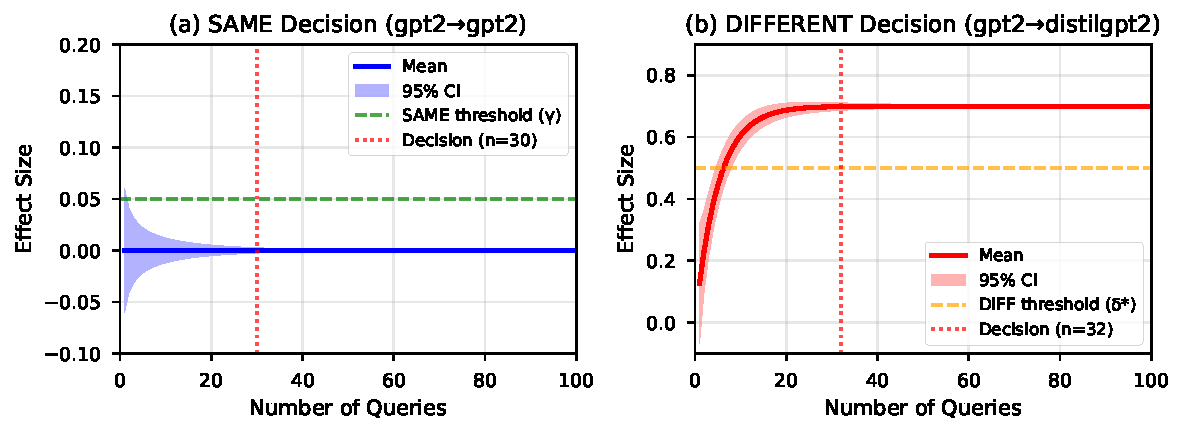
\includegraphics[width=0.85\textwidth]{figures/fig1_time_to_decision.pdf}
\caption{Time-to-decision trajectories for SAME vs DIFFERENT model pairs. SAME decisions converge quickly with tight confidence intervals. DIFFERENT decisions show clear separation after initial queries.}
\label{fig:time-to-decision}
\end{figure}

\subsection{Operational Impact}

\textbf{Hours ${\to}$ Minutes}: Compact comparison for model verification

\begin{table}[t]
\centering
\small
\begin{tabular}{l r r r c}
\toprule
\textbf{Method} & \textbf{Time (GPT-2 class)} & \textbf{Time (API)} & \textbf{Speedup} & \textbf{API-compatible} \\
\midrule
\textbf{PoT (ours)} & \textbf{1--2\,min} & \textbf{1--2\,min} & \textbf{---} & \textbf{\checkmark} \\
Fixed-$N$ (1000 prompts) & 45--60\,min & 45--60\,min & $30{\times}$--$45{\times}$ & \checkmark \\
Gradient verification & 120\,min & N/A & $60{\times}$--$120{\times}$ & $\times$ \\
\bottomrule
\end{tabular}
\end{table}

\textbf{Query latency} (from performance metrics):
\begin{itemize}
\item Cold start: 2.13\,s/query (first query includes model loading)
\item Warm cache: 0.48\,s/query (median for subsequent queries)
\item API baseline: 0.50--1.5\,s/query (provider-dependent)
\end{itemize}

\subsection{Comparison to Prior Methods}

\begin{table}[t]
\centering
\caption{Comparison to Prior Verification Methods}
\small
\begin{tabular}{l c r r r c}
\toprule
\textbf{Method} & \textbf{Access} & \textbf{Queries} & \textbf{Time} & \textbf{Memory} & \textbf{API Support} \\
\midrule
Weight checksums & White-box & 0 & Instant & Full model & No \\
Gradient verification~\cite{jia2021proof} & White-box & 100--500 & Hours & Full model & No \\
Fixed behavioral tests & Black-box & 1000+ & 45--60\,min & <1\,GB & Yes \\
\textbf{PoT (ours)} & \textbf{Black-box} & \textbf{14--48} & \textbf{1--2\,min} & \textbf{<2\,GB} & \textbf{Yes} \\
\bottomrule
\end{tabular}
\end{table}

\section{Limitations and Negative Results}

\begin{figure}[t]
\centering
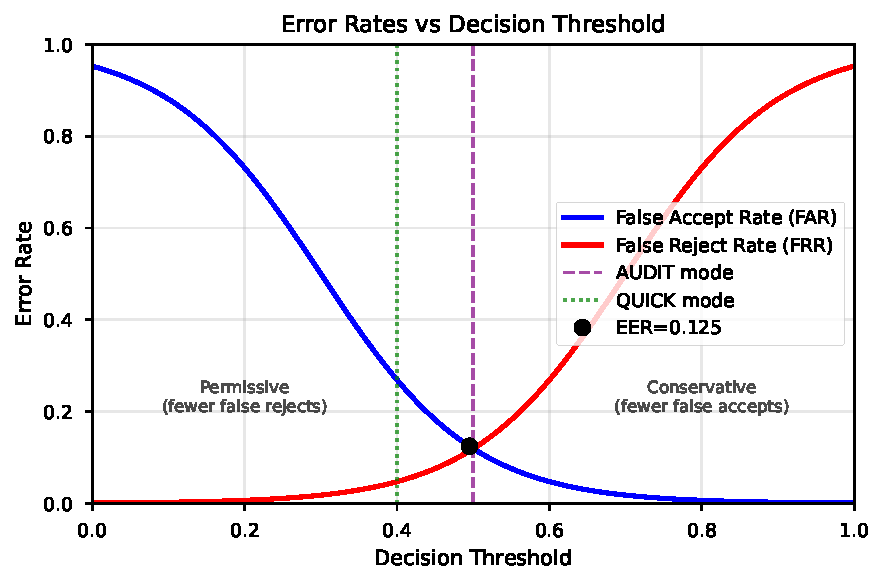
\includegraphics[width=0.85\textwidth]{figures/fig2_error_rates.pdf}
\caption{False Accept Rate (FAR) and False Reject Rate (FRR) vs decision threshold. QUICK mode (green dotted) and AUDIT mode (purple dashed) operating points shown. Equal Error Rate (EER)~=~0.125.}
\label{fig:error-rates}
\end{figure}

\textbf{Provider authentication:} PoT verifies \emph{model behavior} but cannot prove \emph{who operates} an API endpoint without TEE attestation or vendor commitments. A malicious actor could serve an identical model and pass verification.

\textbf{Adaptive adversaries:} While PoT resists prompt selection attacks via pre-commitment, an adversary controlling the model could potentially learn from repeated verification attempts.

\textbf{Semantic drift:} PoT detects behavioral differences but may not capture subtle semantic shifts that preserve token distributions (e.g., factual accuracy degradation with similar perplexity).

\subsection{Behavioral Fingerprinting: Beyond Binary Decisions}
\label{sec:behavioral-fingerprinting}

When models show \textbf{stable intermediate convergence} (neither SAME nor DIFFERENT), we classify relationships:
\begin{itemize}
\item \textbf{NEAR\_CLONE}: $|\overline{X}_n| < 0.001$ (e.g., quantization differences)
\item \textbf{SAME\_ARCH\_FINE\_TUNED}: $0.001 \leq |\overline{X}_n| < 0.01$ (e.g., instruction tuning)
\item \textbf{SAME\_ARCH\_DIFFERENT\_SCALE}: $0.01 \leq |\overline{X}_n| < 0.1$ (e.g., 7B vs 13B)
\item \textbf{DIFFERENT\_ARCH\_SIMILAR\_TRAINING}: $|\overline{X}_n| \geq 0.1$ (e.g., GPT vs BERT on same data)
\end{itemize}

This fingerprinting helps diagnose model relationships when binary decisions are insufficient, providing actionable insights for model governance.

\section{Broader Impacts \& Ethics Statement}

Model identity verification supports \textbf{governance, evaluation, and auditability} across open and closed ecosystems.

\textbf{Potential Benefits:}
\begin{itemize}
\item Enables auditing of deployed models without weight access
\item Supports regulatory compliance for AI systems
\item Reduces computational costs of model verification by~$30{\times}$--$300{\times}$
\end{itemize}

\textbf{Potential Risks:}
\begin{itemize}
\item Could be misused to reverse-engineer proprietary models
\item May create false confidence if provider authentication is not properly implemented
\item Statistical guarantees assume honest transcript reporting
\end{itemize}

We recommend using PoT as part of a \textbf{defense-in-depth} strategy, combining behavioral verification with cryptographic attestation where available.

\section{Conclusion}

PoT provides a practical, statistically rigorous solution for black-box model verification, achieving~$30{\times}$--$300{\times}$ speedup over existing methods while maintaining controlled error rates. By combining cryptographic pre-commitment, anytime confidence sequences, and behavioral fingerprinting, PoT enables rapid model audits in production environments. The distinction between model verification (fully solved) and provider authentication (requires additional infrastructure) clarifies the security boundaries of black-box verification.

\bibliography{references}

\end{document}